                        %%%%%   PREAMBLE  %%%%%

\documentclass[11pt,spanish,a4paper,twoside]{article}

\usepackage[spanish,activeacute,es-noindentfirst]{babel}   % es-noindentfirst: no activa la sangr�a del primer p�rrafo tras un t�tulo
\usepackage{amssymb,amsfonts}
\usepackage{amsmath}             %  Para las f�rmula matem�ticas
\usepackage[latin1]{inputenc}    %  Permite escribir los acentos

\usepackage{fancyhdr}
\renewcommand{\headrulewidth}{0pt}  %  l�nea horiz. bajo el encabezado
\renewcommand{\footrulewidth}{0pt}  %  l�nea horiz. sobre el pie

\usepackage{makeidx}

% \usepackage{times}
% \usepackage[OT1,T1]{fontenc}

\usepackage{palatino}
% palatino: una fuente excelente, pero si sale
% mal en el .pdf descomentar las dos l�neas anterires
% y comentar �sta.

% \usepackage{charter}

\usepackage{vmargin}
\setpapersize{A4}
\setmarginsrb{2.5cm}{2cm}{2.5cm}{2cm}%
{1cm}{1cm}%
{1cm}{1cm}


\usepackage{graphicx}
\usepackage{color}       % Para el color de las fuentes
% \usepackage{lettrine}    % Letra capital
\usepackage{enumerate}   % Entorno enumerate mejorado
\usepackage{mdwlist}     % Entorno descripcion mejorado
\usepackage[amsthm,hyperref,thref]{ntheorem}
%\usepackage{paralist}


\parskip 0.15cm          % Queda mejor pero mas paginas

                        %%%%%   HYPERREF  %%%%%

\usepackage{hyperref}        %  Hiperv�nculos
\hypersetup{                 %  Hiperv�nculos setup
    bookmarksopen=false,
    bookmarksnumbered=true,
    pdfpagemode=UseOutlines,  % None, UseThumbs, UseOutlines (show bookmarks), FullScreen
    colorlinks=true,     % color link text, not a box around them.
    linkcolor=black,      % color for normal internal links.
    anchorcolor=black,   % color for anchor text.
    citecolor=blue,      % color for bibligraphical citations in text.
    filecolor=black,     % color for URLs which open local files.
    menucolor=black,     % color for Acrobat menu items.
%     pagecolor=black,     % color for links to other pages.
    urlcolor=blue,      % color for linked URLs.
    breaklinks=false,    % Allows link text to break across.
    pdfstartview={FitBH},
    pdfview={FitBH},
    %hyperindex=true,
    pageanchor=false
}

% Para el �ltimo
% En realidad, no pasa eso, pero si no pongo "false" tira errores.
%    Determines whether every page is given an implicit
%    anchor at the top left corner. If this is turned off,
%    \tableofcontents will not contain hyperlinks.

% El pen�ltimo me tira un warning pero dejarlo sin comentar     % Hiperreferencias

\usepackage{url}

% \usepackage{longtable}
% \usepackage{supertabular}


% \usepackage{tikz}
% \usepackage{pgf}
% \usepackage{wrapfig}

% \usepackage{placeins}   % Placeins.sty keeps floats "in their place", preventing them from floating past
                        % a "\FloatBarrier" command into another section. To use it, declare
                        % "\usepackage{placeins}" and insert "\FloatBarrier" at places that floats
                        % should not move past, perhaps at every "\section" (en "command.tex")

%% Entorno Descripci�n. En tres sabores:
    %% 1. El m�s general
    \newenvironment{descripcion}[2]%
    {\begin{basedescript}{\desclabelwidth{#2}}%
    \item[#1]}%
    {\end{basedescript}}%

    %% 2. Como poner en negrita (tambi�n parecido a section* pero puedo seguir en la misma l�nea)
    \newenvironment{descripcion0}[1]%
    {\begin{basedescript}{\desclabelwidth{-1ex}}%
    \item[#1]}%
    {\end{basedescript}}%

    %% 3. Con 1.25cm de tama�o
    \newenvironment{descripcion1}[1]%
    {\begin{basedescript}{\desclabelwidth{1.25cm}}%
    \item[#1]}%
    {\end{basedescript}}%

    %% Entorno para citar texto, 80% del tama�o (10% de cada lado)
      \newenvironment{citetext}{%
      \def\leftmargini{0.1\textwidth}%
      \def\rightmargini{0.1\textwidth}%
      \vspace*{-0.35cm}%
      \begin{quotation}\parskip 0.15cm\guillemotleft}%
      {\guillemotright\end{quotation}\vspace*{0.1cm}}


      %% Sin � (caso especial de citetext)
      \newenvironment{citetext_sin_right}{%
      \def\leftmargini{0.1\textwidth}%
      \def\rightmargini{0.1\textwidth}%
      \vspace*{-0.35cm}%
      \begin{quotation}\parskip 0.15cm\guillemotleft}%
      { \end{quotation}\vspace*{0.1cm}}



\newcommand{\subsubseccion}[1]{\subsubsection*{#1}\addcontentsline{toc}{subsubsection}{#1}}




\newcommand{\cleartoevenpage}{%   Similar a \cleardoublepage
    \clearpage
    \ifodd\thepage
        \newpage
    \else
        \newpage
        ~ \\
        \newpage
    \fi
}




\newcommand{\refEQ}[1]{{\color{red} (\ref{#1})}}


\makeindex

\begin{document}
    \pagestyle{headings}
                                           %%% TITULO %%%

\pagestyle{empty}   % para que no tenga n�mero
                    % (�ste es el motivo por el
                    %  cu�l no uso "\maketitle")

% \vspace*{-1.65 cm}
 \begin{center}
   \begin{Large}
%          Online Mathematical Handwriting Recognition
         \textbf{Online Handwriting Recognition}
   \end{Large}
 \end{center}


\vspace*{1.65 cm}
\begin{center}
  \begin{Large}
    \textit{Tesina de Grado
    \vspace*{0.1 cm} \\
    \begin{footnotesize}Agosto 2011    \end{footnotesize}
    }
  \end{Large}
\end{center}


\vspace*{1.65 cm}
\begin{center}
  \begin{Large}
   \textsc{Pablo Speciale}
  \end{Large}
\end{center}


\vspace*{1.65 cm}
\begin{center}
    
\includegraphics[scale=0.04]{imagen/logo_fceia.pdf}
    \hspace*{5cm}
    
\includegraphics[scale=0.25]{imagen/logo_unr.pdf}
\end{center}


\vspace*{0.65 cm}
\begin{center}
\textit{
Lic. en Cs. de la Computaci�n \\
Facultad de Ciencias Exactas, Ingenier�a y Agrimensura \\
Universidad Nacional de Rosario}
\end{center}


\vspace*{3.5cm}
\textbf{Director}: Dr. Juan Carlos Gomez\footnote{Director del grupo \textit{Procesamiento de Se�ales Multimedia} del CIFASIS}

% \vspace{0.5cm}
\textbf{Co-director}:  Dr. Pablo Granitto\footnote{Director del grupo \textit{Aprendizaje Automatizado y Aplicaciones} del CIFASIS}


\newpage




% 
% 
% \topmargin 0 truecm
% 
% \pagestyle{empty}
% 
% \begin{center}
% 
% \vskip -3.0cm
% {\LARGE \sf {\huge mcBrief}: un descriptor local de features \\ para im�genes color} \\
% 
% \vspace{4.0cm}
% {\Large \sf Tesina de grado}
% 
% \vspace{1.5cm}
% {\Large Autor: Daniel Moreno}
% 
% \vspace{0.5cm}
% {\Large Director: Mario E. Munich}
% 
% \vspace{2.4cm}
% {\large \sf Julio 2011}
% 
% \vspace{2.5cm}
% 
% \begin{figure}[h]
% \begin{center}
% \includegraphics[height=1.6cm]{logo_lcc.png}
% \end{center}
% \end{figure}
% 
% \begin{figure}[h]
% \begin{center}
% \includegraphics[height=1.6cm,width=1.6cm]{LogoUNR.png}
% \end{center}
% \end{figure}
% 
% 
% {\it Lic. en Cs. de la Computaci�n \\
% Facultad de Ciencias Exactas, Ingenier�a y Agrimensura \\
% Universidad Nacional de Rosario }
% 
% 
% \end{center}
                            %%%%%   INDICE  %%%%%

\setcounter{page}{1}
\thispagestyle{empty}
\pagenumbering{roman}        % N�meros de p�ginas en Romano

\pagestyle{fancy}
\fancyhf{}                   % Borrar todos los ajustes
\fancyhead[RO,RE]{\scshape{\thepage}}
\fancyhead[LO]{\scshape{�ndice General}}
\fancyhead[LE]{\scshape{�ndice General}}

\pdfbookmark[0]{�ndice General}{tit}       %Agrega "�ndice General"' al bookmark.

\tableofcontents
\clearpage
                            %%%%%   ESTILO  %%%%%

\renewcommand{\headrulewidth}{0pt}  %  l�nea horiz. bajo el encabezado
\renewcommand{\footrulewidth}{0pt}  %  l�nea horiz. sobre el pie

\pagenumbering{arabic}

%
%  Simple faz
%
\pagestyle{fancy}
\fancyhf{}                   % Borrar todos los ajustes
\fancyfoot[C]{\thepage}
% \fancyhead[RO,RE]{\scshape{\thepage}}  % N�meros de p�gina en las esquinas de los encabezados
\renewcommand{\sectionmark}[1]{
    \fancyhead[RO]{\begin{footnotesize}\thesection.\ \scshape{#1}\end{footnotesize}}
    \fancyhead[RE]{\begin{footnotesize}\thesection.\ \scshape{#1}\end{footnotesize}}
    \renewcommand{\headrulewidth}{0.1pt}
}
\renewcommand{\subsectionmark}[1]{
    \fancyhead[RE]{\begin{footnotesize}\thesubsection.\ \scshape{#1}\end{footnotesize}}
}


%
%  Doble faz
%
% \pagestyle{fancy}
% \fancyhf{}                   % Borrar todos los ajustes
% \fancyfoot[C]{\thepage}
% % \fancyhead[RO,LE]{\begin{small}\thepage\end{small}}  % N�meros de p�gina en las esquinas de los encabezados
% \renewcommand{\sectionmark}[1]{
%     \fancyhead[RO]{\begin{footnotesize}\thesection.\ \scshape{#1}\end{footnotesize}}
%     \fancyhead[LE]{\begin{footnotesize}\thesection.\ \scshape{#1}\end{footnotesize}}
%     \renewcommand{\headrulewidth}{0.1pt}
% }
% \renewcommand{\subsectionmark}[1]{
%     \fancyhead[RE]{\begin{footnotesize}\thesubsection.\ \scshape{#1}                   \end{footnotesize}}
% }


%% Para los perzonalizar itemize
\renewcommand{\labelitemi}{$\bullet$}
\renewcommand{\labelitemii}{$\ast$}


% % A more convenient way to stop floats at section boundaries is to change
% % the definition of "\section" to include "\FloatBarrier", at the beginning
% \let\oldsection\section
% \renewcommand{\section}{\FloatBarrier\oldsection}


% % Util para ser impreso. Hace que las secciones comiencen desde una p�gina impar
% % similar a \cleardoublepage
% \let\oldsection\section
% \renewcommand{\section}{\cleartoevenpage\oldsection}


\let\oldsection\section
\renewcommand{\section}{\clearpage\oldsection}


\def\tablename{Tabla} % Cambia "Cuadro" por "Tabla"


% Links internos en rojo
\hypersetup{
    linkcolor=red,
}
    \pagestyle{fancy}

% \titlespacing*{\section}{0pt}{1.5ex}{1.5ex}

%     \section{Introducci�n}

\subsection*{Motivaci�n}
\noindent
Poder escribir en dispositivos electr�nicos es factible actualmente, sobre todo con la llegada de las Tablet PC, pizarras el�ctricas, celulares touch-screen y las pantallas t�ctiles. Tambi�n cabe destacar algunos e-Readers que permiten la escritura, convirti�ndose en \textit{papel electr�nico}. La escritura se realiza generalmente con un \textit{stylus} (l�piz), abriendo la puerta a nuevas interacciones m�s all� del teclado y mouse. En la figura \ref{tabletas}, puede apreciarse una variedad de dispositivos que permiten la escritura con l�piz.
\begin{figure}[!htbp]
 \centering
 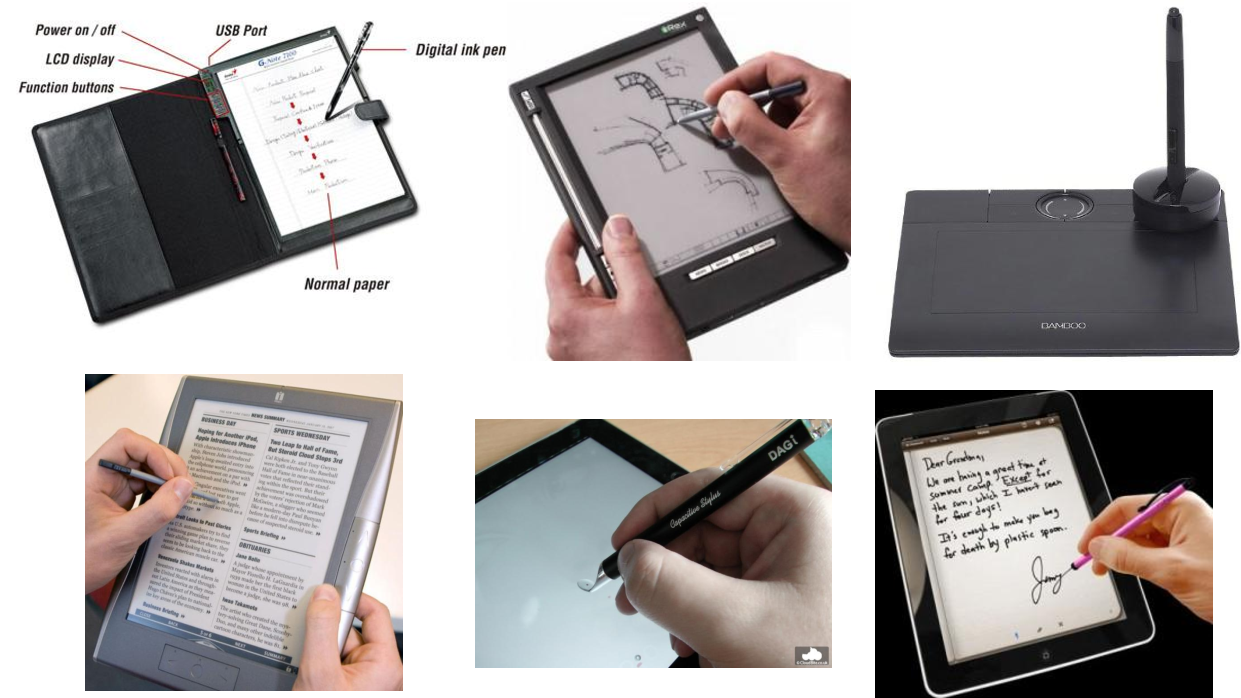
\includegraphics[scale=0.70]{imagen/tabletas.pdf}
 \caption{Tabletas}
 \label{tabletas}
\end{figure}


\vspace*{-1ex}
\subsection*{Online vs Offline Recognition}
\label{Fundamentos}

% \subsubsection*{On-line vs Off-line}
\noindent
A diferencia del enfoque \textit{Offline} de handwriting recognition, el cual pretende reconocer caracteres a partir de una imagen, el enfoque \textit{Online} intenta el reconocimiento a partir de trazos. Ambos enfoques est�n esquem�ticamente representados en la figura \ref{fig:off|on-line}.
\begin{figure}[!htbp]
 \centering
 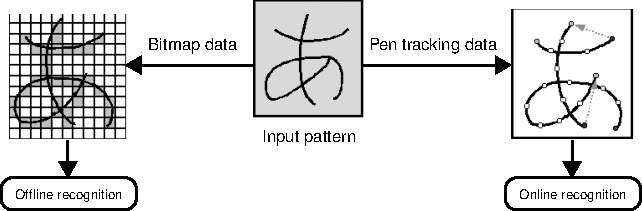
\includegraphics[scale=0.85]{imagen/off|on-line.pdf}
 \caption{Offline vs Online.}
 \label{fig:off|on-line}
\end{figure}

Como puede verse, se posee el orden en que cada uno de los puntos fue escrito. As�, es posible diferenciar distintos estilos de escrituras, a pesar de que el resultado final puede que sea el mismo. . La utilizaci�n de un stylus en un dispositivo electr�nico permite usar el enfoque online.



\subsubsection*{Handwriting recognition}
\noindent
En el an�lisis de Handwriting para contenido matem�tico se reconocen 4 etapas, como se destaca en \cite{CommunicatingMathematics}:
% colecci�n de trazos (digital ink), reconocimiento de caracteres, an�lisis estructural y determinaci�n de sem�ntica.

\begin{enumerate}[A.]

 \item \textbf{Colecci�n de trazos}

Un caracter puede ser escrito con un s�lo trazo (\textit{Single-Stroke}) o con muchos (\textit{Multi-Stroke}), ver figura \ref{fig:single|multi-stroke}. El problema de determinar qu� trazos pertenecen a qu� caracteres es llamado \textit{Stroke grouping}.
\begin{figure}[!htbp]
 \centering
 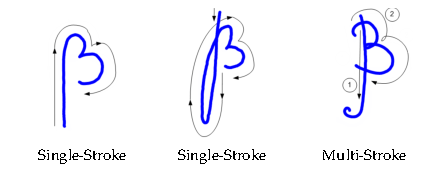
\includegraphics{imagen/single|multi-stroke.pdf}
 \caption{Izquierda y centro caracter Single-Stroke. Derecha Multi-Stroke.}
 \label{fig:single|multi-stroke}
\end{figure}


 \item \textbf{Reconocimiento de caracteres}

El reconocimiento tiene 3 etapas:
    \begin{enumerate}[1.]
    \item \textit{Preproceso}

    El preprocesado primero elimina el ruido frecuentemente presente al principio y final de cada trazo. Luego, se normaliza por \textit{resampling} y \textit{resizing}. Resampling ayuda a unificar distancias entre los puntos, y resizing asegura que el tama�o del caracter escrito no afecte al resultado del reconocimiento.

    \begin{figure}[!htbp]
    \centering
    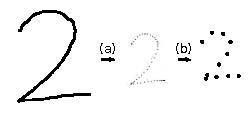
\includegraphics{imagen/preprocesing.pdf}
    \label{fig:preprocesing}
    \caption{(a) Suavizado y resizing, (b) luego resampling }
    \end{figure}


    \item \textit{Extracci�n de caracter�sticas (Feature extraction)}

    En este paso se extraen caracter�sticas (feature) de los trazos. Hay varios tipos de features: los relativos a apariencia que incluye, por ejemplo, proporci�n entre la altura y ancho; los relativos a propiedades geom�tricas, como ser la cantidad de loops e intersecciones; los relativos al estilo de escritura, como la direcci�n y cantidad de strokes.

    Estos features son usados como criterio para podar el �rbol de modelos, dejando una cantidad peque�a de clases a examinar, incrementando la performance del reconocimiento. Por ejemplo, en el caso de escribir ``$\ell$'' o ``$\alpha$'', solo se considerar�n los modelos que contienen un �nico loop.


    \item \textit{Matching}

    La etapa final del reconocimiento es el matching de la entrada con los modelos en una base de datos. Despu�s de que los features podaron el �rbol de modelos, es necesario lidiar con solo una fracci�n de la colecci�n. Se pueden citar algoritmos como \textit{Elastic Matching} \cite{ElasticMatching} o \textit{Legendre-Sobolev} \cite{LegendreSobolevComp, OnlineStrokeModeling}.

    \end{enumerate}


% \newpage
    \item \textbf{An�lisis estructural}

Como la entrada se espera que sea matem�tica, adem�s de reconocer cada caracter individual, tambi�n se tienen que interpretar su posici�n y rol en la expresi�n. Primero, se considera solo la posici�n relativa de los caracteres, sin determinar su sem�ntica, como se ve en el ejemplo representado en la figura \ref{fig:layout_trees}.
\begin{figure}[!htbp]
 \centering
 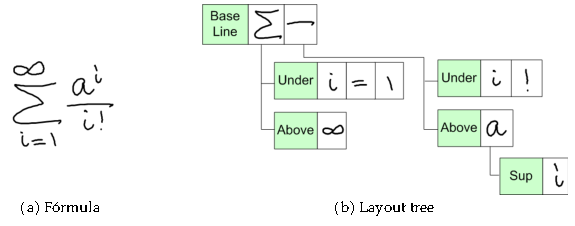
\includegraphics{imagen/layout_trees.pdf}
 \caption{Representaci�n de la f�rmula manuscrita y su correspondiente Layout.}
 \label{fig:layout_trees}
\end{figure}

Luego, se marcan expl�citamente decimales, operadores, fracciones, etc. Cada nodo en el �rbol es asignado a un rol en la expresi�n. Se intenta distinguir entre nombres de funciones y de variables, entre multiplicaciones impl�citas de aplicaci�n de funciones, etc. %Esta etapa es dif�cil y requiere sem�ntica profunda.



\item \textbf{Extracci�n de contenido matem�tico}

El �rbol construido despu�s del an�lisis estructural ya posee sem�ntica y puede ser transformado directamente a \LaTeX~ o MathML \cite{MathML}.


\end{enumerate}


    \section{Conceptos Generales}
\label{sec:Conceptos_Generales}

En esta secci�n se describir�n las partes esenciales de sistema de reconocimiento de escritura manuscrita, permitiendo as� aclarar en d�nde se centrar� este trabajo. Tambi�n se comentar�n brevemente las etapas que intervienen en el proceso de reconocimiento de escritura.
% que tiene un sistema de reconocimiento de escritura.


% En esta secci�n describir las partes esenciales del campo y reducirlo para
% ubicar al lector para que pueda entender en que parte del campo se trabaj�.

% se intenta reducir el campo de handwriting recognition de manera que se pueda apreciar en qu� parte del campo se est� trabajando. Tambi�n se describen las etapas en las cu�les se debe profundizar.

% se centralizar�
% para centrarlo en un subdominio

% focalizar�
% reducir�


\vspace*{-1ex}
\subsection{Reconocimiento Online vs Offline}
\label{Fundamentos}

% \subsubsection{On-line vs Off-line}
% \noindent
A diferencia del enfoque \textit{Offline} de handwriting recognition, el cual pretende reconocer caracteres a partir de una imagen, el enfoque \textit{Online} intenta el reconocimiento a partir de secuencias de puntos, aqu� llamados trazos (\textit{strokes}). Ambos enfoques est�n esquem�ticamente representados en la figura \ref{fig:off|on-line}.
\begin{figure}[!htbp]
 \centering
 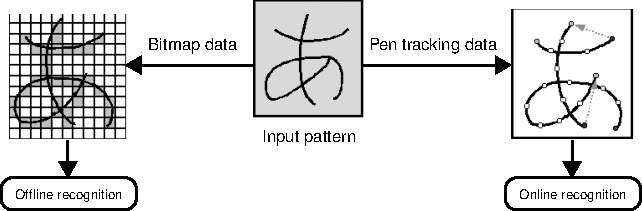
\includegraphics[scale=0.85]{imagen/off_vs_on-line.pdf}
 \caption{Offline vs Online.}
 \label{fig:off|on-line}
\end{figure}

Como puede verse, en el enfoque, se conoce el orden en que cada uno de los puntos fue escrito. As�, es posible diferenciar distintos estilos de escrituras, a pesar de que el resultado final puede que sea el mismo. La utilizaci�n de un stylus en un dispositivo electr�nico permite usar el enfoque Online.


\subsection{Segmentaci�n}
\label{segmentation}
% \noindent
En el presente trabajo, se asume que la escritura est� en imprenta y que los s�mbolos est�n bien distanciados entre s�. En la figura \ref{fig:segmentation}, se muestran distintos niveles de dificultad en la segmentaci�n, variando desde el caso m�s simple (el ya segmentado, caso 1) hasta el caso m�s complejo (mezcla de escritura cursiva e imprenta, caso 5). Se considera el caso 2 para la construcci�n de la base de datos. Los niveles superiores de escritura requieren de un trabajo adicional de segmentaci�n que no entra en el alcance de este trabajo.
\begin{figure}[!htbp]
 \centering
 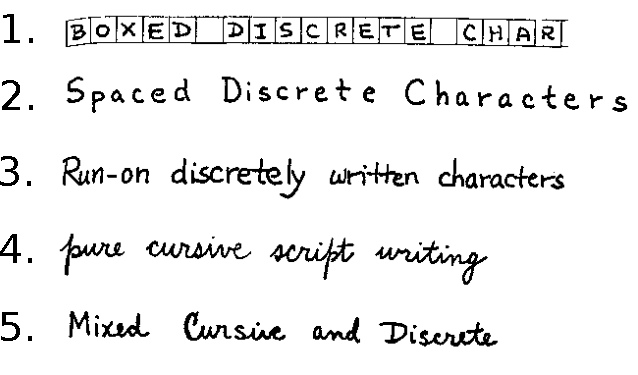
\includegraphics[scale=0.70]{imagen/segmentation.pdf}
 \caption{Niveles de dificultad en segmentaci�n \cite{Connell00onlinehandwriting}.}
 \label{fig:segmentation}
\end{figure}



\subsection{Etapas del Reconocimiento de Escritura}
\noindent
En el an�lisis de escritura manuscrita se pueden reconocerse las siguientes posibles etapas:
% , como en parte se destaca en \cite{CommunicatingMathematics}:


\subsubsection{Colecci�n de trazos}
Un s�mbolo\footnote{Se usa el t�rmino \textit{s�mbolo} en vez de \textit{caracter} pues puede ser un d�gito, una letra o un s�mbolo matem�tico.} puede ser escrito con un s�lo trazo (\textit{Single-Stroke}) o con muchos (\textit{Multi-Stroke}), ver figura \ref{fig:single|multi-stroke}. El problema de determinar qu� trazos pertenecen a qu� caracteres es llamado \textit{Stroke grouping}. Observar que esta etapa depende de la segmentaci�n asumida, ver secci�n~\ref{segmentation}.
\begin{figure}[!htbp]
 \centering
 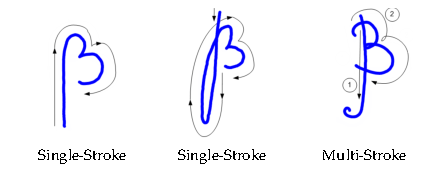
\includegraphics{imagen/single_vs_multi-stroke.pdf}
 \caption{Los dos primeros trazos son Single-Stroke, y el �ltimo es Multi-Stroke.}
 \label{fig:single|multi-stroke}
\end{figure}


 \subsubsection{Preproceso}
 \label{sec:conceptos_preproceso}
    En el preprocesado pueden aplicarse diferentes tipos de filtros. El \textit{suavizado} elimina el ruido frecuentemente presente al principio y final de cada trazo. La normalizaci�n por \textit{resampling} ayuda a unificar distancias entre los puntos, y la normalizaci�n por \textit{resizing} asegura que el tama�o del caracter escrito no afecte al resultado del reconocimiento. En la figura \ref{fig:preprocesing} puede observarse una posible secuencia de aplicaci�n de filtros.

    \begin{figure}[!htbp]
    \centering
    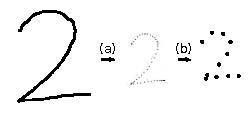
\includegraphics{imagen/preprocesing.pdf}
    \caption{\texttt{(a)} Suavizado y Resizing, \texttt{(b)} Resampling }
    \label{fig:preprocesing}
    \end{figure}


 \subsubsection{Extracci�n de caracter�sticas (\textit{Feature extraction})}
    En este paso se extraen caracter�sticas (\textit{features}) de los trazos. Hay varios tipos de features que se han usado tradicionalmente: los relativos a la apariencia que incluye, por ejemplo, proporci�n entre altura y ancho; los relativos a propiedades geom�tricas, como ser la cantidad de loops e intersecciones, centro de gravedad, puntos dominantes; los relativos al estilo de escritura, como la direcci�n y cantidad de strokes. Se posterga para la secci�n~\ref{feature_extraction} la explicaci�n de los features utilizados en este trabajo.


 \subsubsection{Entrenamiento (\textit{Training})}
    Se requiere tener una base de datos de modelos con la cual contrastar el s�mbolo actual de entrada. Se realiza por una �nica vez en los algoritmos que permiten entrenamiento.
%     Y si se quiere pensarlo as�, realmente esta etapa no es parte del reconocimiento de la entrada actual en s�.


 \subsubsection{Reconocimiento o Estimaci�n (\textit{Matching})}
    Aqu� se intenta estimar, para la entrada actual, cu�l modelo es el m�s ``similar'', sobre la base de datos disponible que sirvi� de entrenamiento. Es decir, se clasifica a la nueva entrada determinando a qu� clase pertenece. Pueden considerarse m�ltiples estimaciones, por ejemplo, dar las mejores tres estimaciones; pero en este trabajo solo se considera la primera (\textit{first match}).



\subsection{Dependiente o independiente del usuario}
    Un sistema de \textit{handwriting recognition} puede ser dividido en: dependiente del usuario (\textit{writer-dependent}) o independiente del usuario (\textit{writer-independent}). Un sistema \textit{writer-independent} es entrenado para reconocer una gran variedad de estilos de escritura, mientras que un sistema \textit{writer-dependent} es entrenado para reconocer a un �nico individuo. Un sistema \textit{writer-dependent} trabaja con datos con poca variabilidad, y entonces puede alcanzar mejores resultados, el �nico problema es que exige al usuario tomarse el tiempo para entrenar el sistema.

    En este trabajo se pueden utilizar ambos enfoques, dependiendo de la base de datos utilizada.


    \section{Fundamentos}
\label{fundamentos}

En esta secci�n se introducir� algunos conceptos b�sicos que utilizaremos a lo largo del trabajo.


\subsection{Preliminares}

Sea una familia de funciones $\{B_i\}$ en el espacio de funciones continuas en $[a,b]$, se definen

\begin{descripcion1}{Producto interno:}
\begin{align}
\label{def:inner_product}
 \langle B_i, B_j \rangle & \doteq \int_{a}^{b}{B}_{i}(t) \,{B}_{j}(t) \, w(t) dt
\end{align}
\end{descripcion1}

\begin{descripcion1}{Norma:}
\begin{align}
\label{def:norma}
 \| B_i \| & \doteq \sqrt{ \langle B_i, B_i \rangle }
\end{align}
\end{descripcion1}

\begin{descripcion1}{Kronecker delta:}
\begin{align}
\delta_{ij} =
        \left\{
            \begin{array}{ll}
                1 & \mbox{si } i = j \\
                0 & \mbox{si } i \neq j
            \end{array}
        \right.
\end{align}
\end{descripcion1}

\subsubsection*{Ortogonalidad:}
Se dicen que $B_i$ y $B_j$ son ortogonales si se cumple que $\langle B_i, B_j \rangle = 0$

\subsubsection*{Ortogonalizaci�n de Gram-Schmidt:}
Sea $\{v_1, \dots, v_n\}$ una base de un espacio $U$ con producto interno, se define recursivamente
\begin{align}
\label{eq:Gram-Schmidt}
u_i & = \left( v_i - \sum_{i=0}^{i-1}{\langle v_i, u_j\rangle u_j} \right)
\end{align}
Entonces, $\{u_1, \dots, u_n\}$ una base ortogonal y $\left\{\frac{u_1}{\|u_1\|}, \dots, \frac{u_n}{\|u_n\|}\right\}$ es base ortonormal de $U$.


\subsection{Polinomios ortogonales}
Polinomios ortogonales son clases de polinomios $\{B_{i}(t)\}$ definidos sobre el dominio $[a,b]$ que obedecen la relaci�n de ortogonalidad
\begin{align}
\label{eq:ortogonalidad}
\int_{a}^{b}{B}_{i}(t) \,{B}_{j}(t) \, w(t) dt & = 0 \quad\quad \text{cuando $i \neq$} j
\end{align}
donde $w(t)$ es una funci�n peso. Si adem�s cumplen con
\begin{align}
\label{eq:ortonormalidad}
 \int_{a}^{b}{B}_{i}(t) \,{B}_{j}(t) \, w(t) dt & = \delta_{ij}
\end{align}
los polinomios son \textit{\textbf{ortonormales}}. Es decir, est�n normalizados: $ \| B_i \| = 1$


% La tabla \ref{table:polinomios} muestra algunos ejemplos de los polinomios ortogonales: \\
% \begin{table}[!htbp]
% \centering
%     \begin{tabular}{ | l |c |c | c |}
%     \hline
%     \hline
%     \textbf{Polinomio} & dominio & $w(t)$ & $c_{n}$ \\
%     \hline
%     Chebyshev  & $[-1,1]$ & $(1-t^2)$ & $  $ \\[1ex]
%     Legendre   & $[-1,1]$ & $1$       & $ \frac{2}{2\,n+1} $ \\[1ex]
%     Jacobi     & $(-1,1)$ & $(1-t)^{\alpha}\,(1+t)^{\beta}$ & $ $ \\[1ex]
%     \hline
%     \hline
%     \end{tabular}
% \label{table:polinomios}
% \caption{Ejemplos de polinomios ortogonales}
% \end{table}




\subsubsection{Polinomios de Legendre}
\label{legendre}
% Son polinomios ortogonales definidos en $[-1,1]$. Se sabe que el grado de $L_i$ es exactamente $i$,  entonces pueden escribirse como

Si tomamos como funci�n peso $w(t)=1$ en la definici�n \refEQ{def:inner_product} de producto interno, es decir,
\begin{align*}
 \langle L_i, L_j \rangle & = \int_{-1}^{1}{L}_{i}(t) \,{L}_{j}(t)\,w(t)\,dt = \int_{-1}^{1}{L}_{i}(t) \,{L}_{j}(t)\,dt
\end{align*}
se pueden generar los polinomios de Legendre $\{L_i\}$ con el proceso de ortogonalizaci�n de Gram-Schmidt \refEQ{eq:Gram-Schmidt} en el intervalo $[-1,1]$. Normalizando de tal manera que $L_n(1)=1$ da los polinomios de Legendre esperados. Algunos de ellos:
\begin{align*}
L_0(t) &= 1 \\[1ex]
L_1(t) &= t \\
L_2(t) &= \frac{3\,{t}^{2}-1}{2} \\
L_3(t) &= \frac{5\,{t}^{3}-3\,t}{2} \\
L_4(t) &= \frac{35\,{t}^{4}-30\,{t}^{2}+3}{8} \\
 &~ ~\vdots
\end{align*}

% \subsubsection*{Shifted Legendre Polynomials}
Para nuestro prop�sito es conveniente utilizar los polinomios an�logos definido en $[0,1]$, los cuales son llamados \textit{\textbf{shifted} Legendre polynomials},
\begin{align}
\label{eq:legendre}
L_i(t) &= \sum_{j=0}^{i}{ C_{ij}\,x^j }
\end{align}
% donde los coeficientes $C_{ij}$ pueden calcularse con una f�rmula cerrada, ver \cite{abramowitz70a}
el grado de $L_i$ es exactamente $i$.  Se conoce una f�rmula cerrada para el c�lculos de los coeficientes $C_{ij}$ ortonormales. A continuaci�n dicha f�rmula, que puede encontrarse en \cite{abramowitz70a},
\begin{align}
\label{eq:legendre_coefficients}
C_{ij} &= (2\,i+1)^{\frac{1}{2}}\begin{pmatrix}i\cr j\end{pmatrix} {\left( -1\right) }^{j} \begin{pmatrix}j+i\cr j\end{pmatrix}
\end{align}

% \noindent
Pueden verse los primeros diez polinomios de Legendre gr�ficamente en la figura~\ref{fig:legendre}.
\begin{figure}[!htbp]
\vspace*{-0.6cm}
\centering
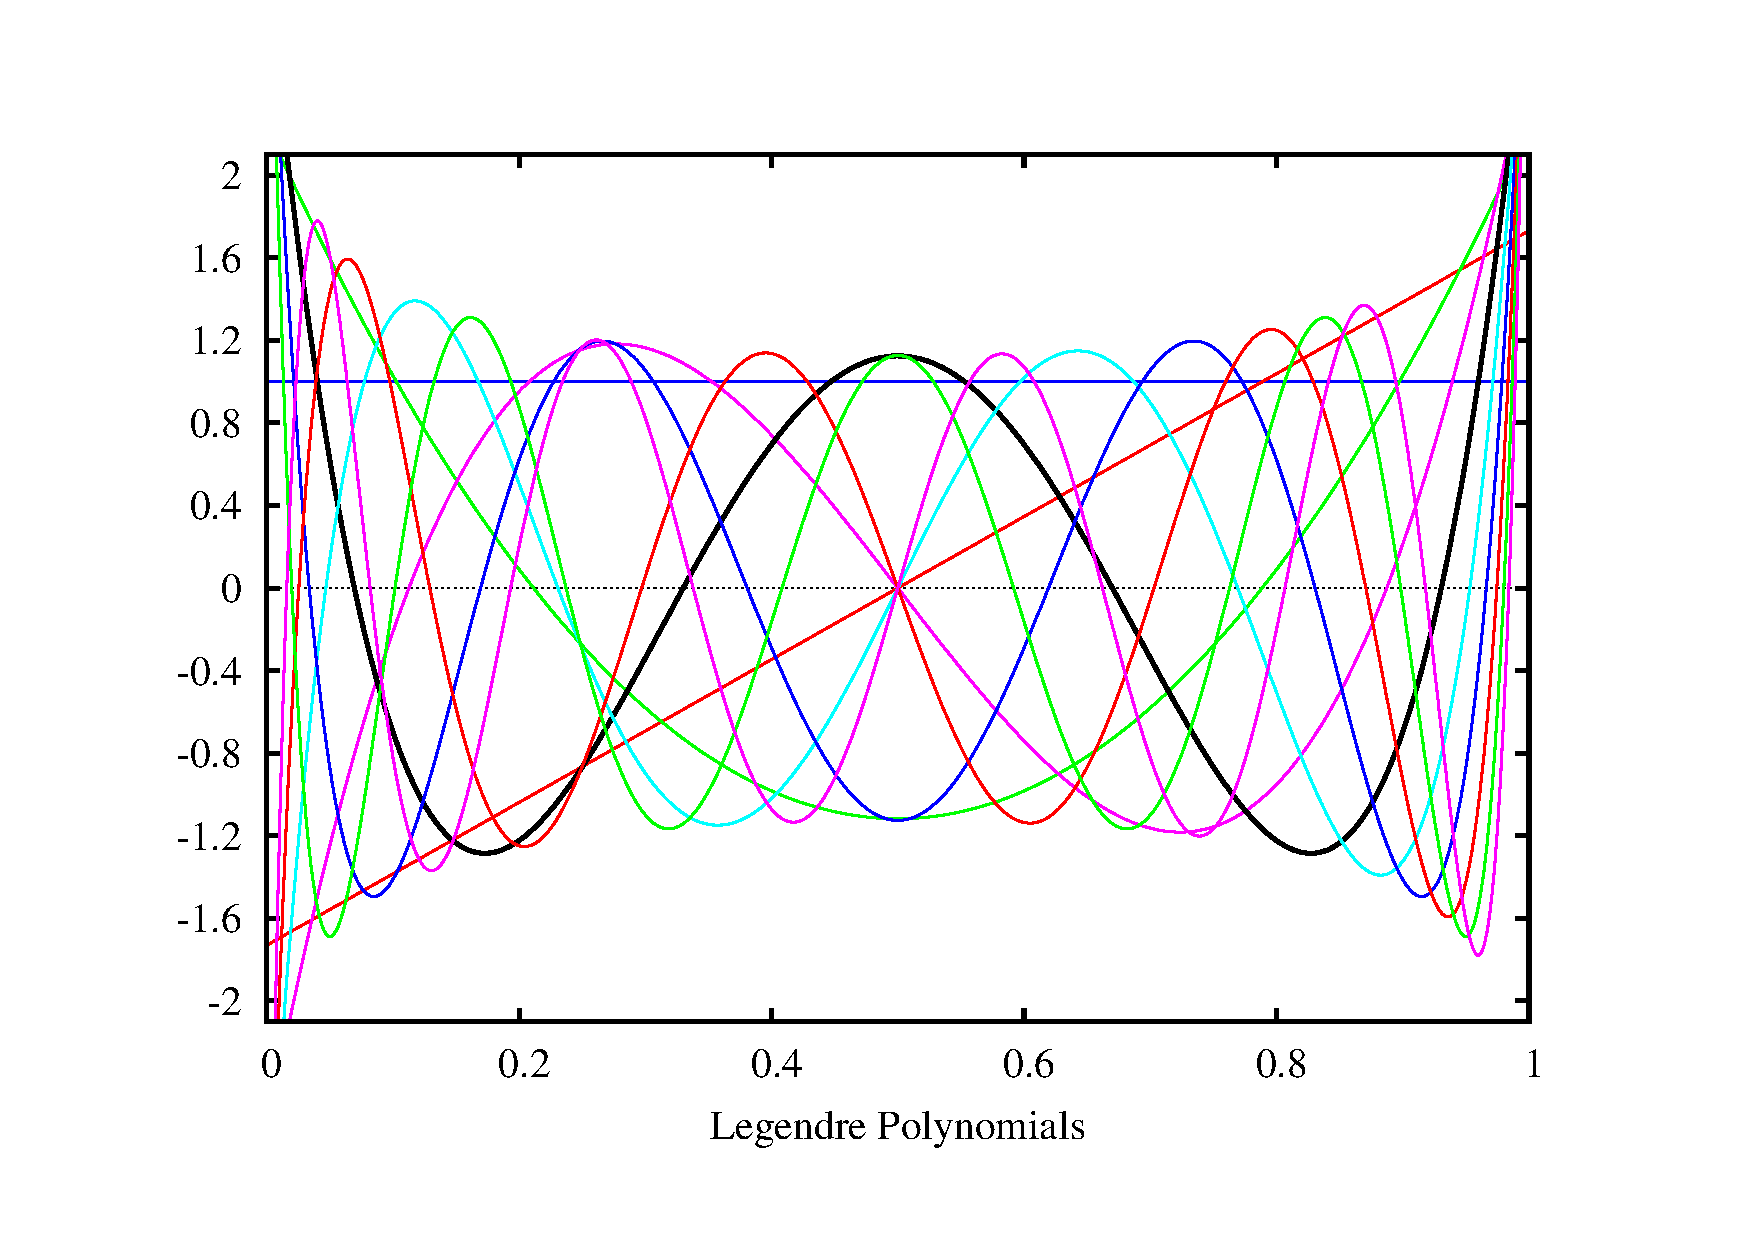
\includegraphics[scale=0.275]{imagen/legendre.pdf}
\vspace*{-0.6cm}
\caption{Primeros diez polinomios de Legendre (shifted) en $[0,1]$}
\label{fig:legendre}
\end{figure}


% \begin{align}
% \begin{split}
% \label{eq:legendre}
% L_i(t) &= \sum_{j=0}^{i}{ C_{ij}\,x^j }\\
% \text{donde} \quad C_{ij} &= (2\,i+1)^{\frac{1}{2}}\begin{pmatrix}i\cr j\end{pmatrix} {\left( -1\right) }^{j} \begin{pmatrix}j+i\cr j\end{pmatrix}
% \end{split}
% \end{align}


\subsubsection{Polinomios de Chebyshev}

(falta)

\subsubsection{Polinomios de Legendre-Sobolev}

(falta)

\subsection{Series de funciones ortogonales}
\label{Series_de_funciones_ortogonales}
\noindent
Si $\{B_i\}$ es una base de polinomios ortonormales respecto al producto interno \refEQ{def:inner_product},
%$L^2[a,b]$,
una funci�n continua~$f$ en el dominio $[a,b]$ puede ser escrita como
\[ f(t) = \sum_{i=0}^{\infty}{\alpha}_{i}\,{B}_{i}(t) \]
Al aplicar el producto interno con $B_i$ en ambos lados de la ecuaci�n anterior se obtiene:
\begin{align*}
\langle f, B_i \rangle & =   \left\langle \sum_{i=0}^{\infty}{\alpha}_{i}\,{B}_{i}(t), B_{i}(t) \right\rangle
                         =   \sum_{i=0}^{\infty} {\alpha}_{i} \langle {B}_{i}, B_i \rangle
                         =   \sum_{i=0}^{\infty} {\alpha}_{i} \delta_{ij}
                         =   {\alpha}_{i}
\end{align*}
Reescribiendo,
\begin{align}
\label{eq:alpha_inner_prod}
{\alpha}_{i} & = \langle f, B_i \rangle
\end{align}
\noindent
Entonces, se puede obtener una aproximaci�n a $f(t)$ al truncar la serie en un cierto orden $d$,
\begin{align}
% \begin{split}
\label{eq:aprox}
f(t) & \approx \sum_{i=0}^{d}{\alpha}_{i}\,{B}_{i}(t)
%      & =  \sum_{i=0}^{d}\langle f, B_i \rangle\,{B}_{i}(t)
\end{align}

    \section{Feature extraction}
\label{feature_extraction}

Las t�cnicas usuales para \textit{handwriting recognition} tratan de encontrar \textit{features} particulares sobre un conjunto de s�mbolos, citemos por ejemplo los d�gitos. Pero al cambiar dicho conjunto, estos features dejan de ser efectivos, no discriminan correctamente. Se vuelve impr�ctico desarrollar heur�sticas para reconocer features espec�ficos para cada s�mbolo.
% Sobre todo si se tiene en cuenta que s�mbolos matem�ticos pueden ser inventados o agregados en la marcha.
Por lo que es deseable buscar una representaci�n que permita ser aplicada sin importar qu� tipo de s�mbolo se trate; ya sea un d�gito, una letra o un s�mbolo matem�tico.

Unos de los mayores problemas con los m�todos de reconocimientos tradicionales es que los trazos son tratados como secuencias de puntos (en \textit{discreto}), en vez de verlos como lo que realmente son, curvas (en \textit{continuo}).
% son pensados como una secuencia de puntos. El problema con �sto es que no se lo est�n tratando como lo que realmente son, curvas.

\subsection{Trazos discretos como curvas continuas}
\label{Trazos_como_curvas_continuas}

En vez de describir a los trazos como una secuencia de puntos, �stos pueden ser representados por aproximaciones de curvas, figura~\ref{fig:trazos_vs_curvas}. Se mostrar� que se necesitan menos de vein\-tes~($20$) coeficientes de una serie para representar un trazo.
% \vspace*{-0.1cm}
    \begin{figure}[!htbp]
    \centering
    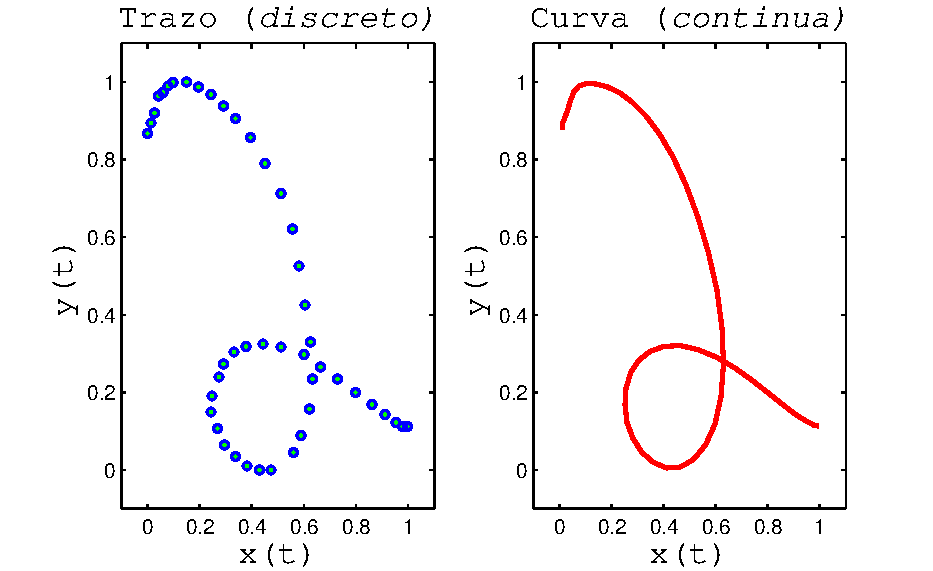
\includegraphics[scale=0.4]{imagen/trazos_como_curva.pdf}
%     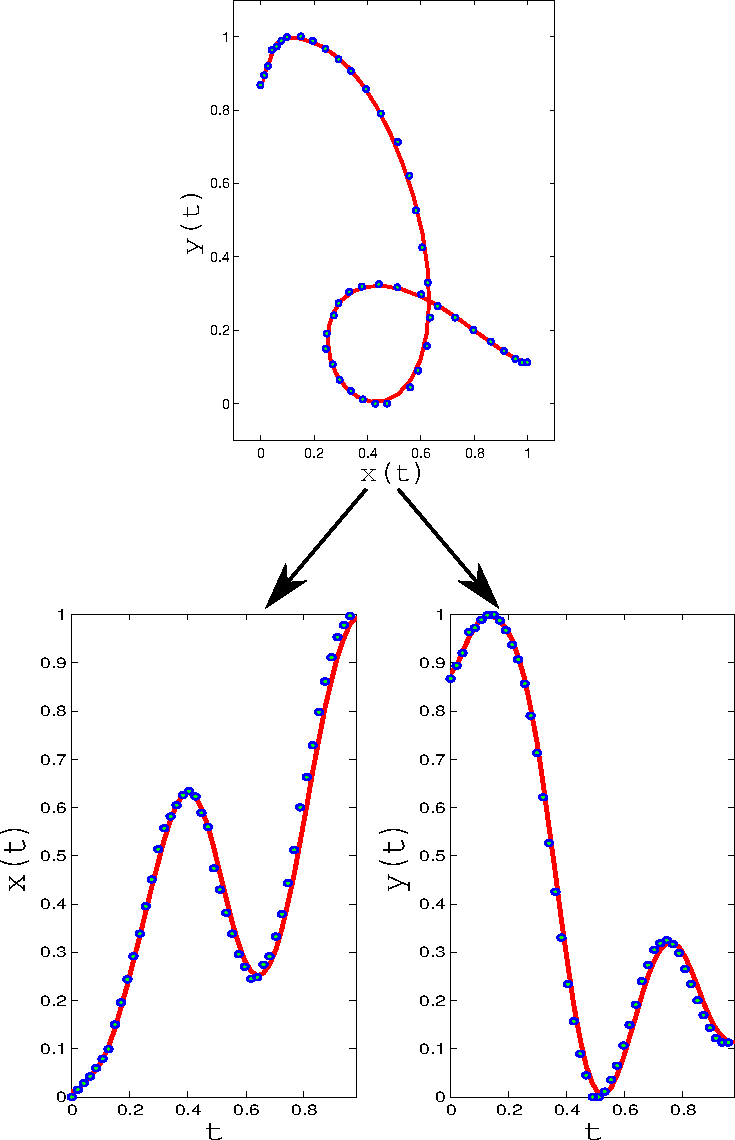
\includegraphics[scale=0.23]{imagen/x_e_y_en_t.pdf}
    \caption{Trazos como curvas param�tricas: $r(t) = \{x(t),y(t)\}$ }
    \label{fig:trazos_vs_curvas}
    \end{figure}

\vspace*{-0.2cm}
\noindent
Observar que se necesitan aproximar dos curvas: $x(t)$, $y(t)$ por s�mbolos, figura~\ref{fig:x_e_y_en_t}.
% \vspace*{-0.15cm}
    \begin{figure}[!htbp]
    \centering
    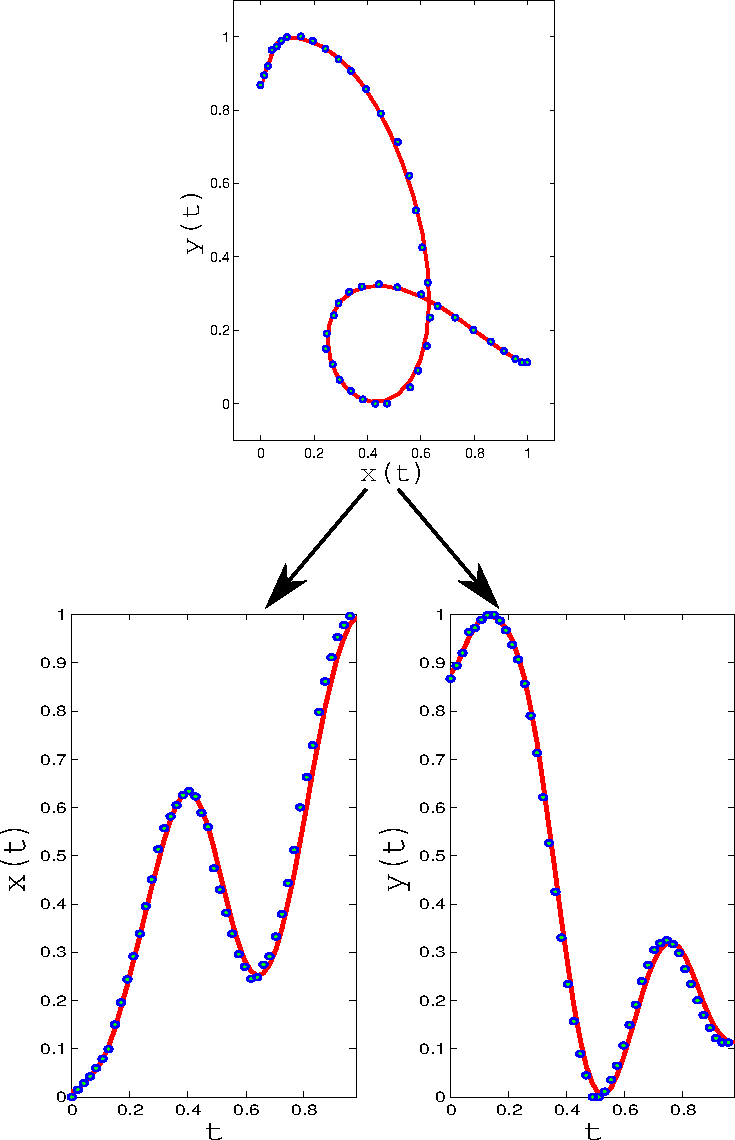
\includegraphics[scale=0.29]{imagen/x_e_y_en_t.pdf}
    \caption{En \textcolor{red}{rojo} las aproximaciones de $x(t)$, $y(t)$}
    \label{fig:x_e_y_en_t}
    \end{figure}

\vspace*{-0.2cm}
\noindent
Trabajos anteriores \cite{Succinct} han demostrado c�mo las coordenadas $x(t)$, $y(t)$ de s�mbolos escritos a mano pueden ser representados como expansi�n en series de polinomios ortogonales de \textit{Chebyshev}; y que los coeficientes de las series truncadas adem�s de ser las aproximaciones buscadas, pueden ser usados para clasificaci�n y reconocimiento.

De manera similar, en este trabajo se utiliza un n�mero finito de \textit{\textbf{momentos matem�ticos}} para la reconstrucci�n de funciones (las curvas) como series truncadas de polinomios ortogonales de \textit{\textbf{Legendre}}, siguiendo las ideas presentadas en los art�culos \cite{Moments} y \cite{OnlineModeling}. Este problema es conocido como \textit{\textbf{Hausdorff Moment Problem}} \cite{HausdorffMomentProblem}. Una alternativa a este m�todo para la obtenci�n de las aproximaciones a las curvas (es decir, los coeficientes de las series truncadas) es utilizar \textit{aproximaci�n por \textbf{m�nimos cuadrados}} a trav�s de la \textit{\textbf{pseudo-inversa} de Moore-Penrose}, permitiendo este enfoque utilizar polinomios ortogonales arbitrarios, en particular polinomios de \textit{\textbf{Legendre}}, \textit{\textbf{Legendre-Sobolev}} y \textit{\textbf{Chebyshev}}.

% usar diferentes tipos de polinomios ortogonales, en particular \textit{\textbf{Legendre}}, \textit{\textbf{Legendre-Sobolev}} y \textit{\textbf{Chebyshev}}.


% En lo siguiente se ir�n introduciendo algunos conceptos para finalmente llegar a la explicaci�n de qu� son los features, y c�mo obtenerlos.


\subsection{Representaci�n con series}
Se desea entonces aproximar las funciones $x(t), y(t)$ de los trazos. Como se indic� en la secci�n~\ref{Series_de_funciones_ortogonales}, �sto puede hacerse como expansi�n de series de polinomios ortogonales; seg�n la ecuaci�n~(\ref{eq:alpha_inner_prod}),
\[
\left\{
\begin{array}{rcl}
% \begin{equation}
% \begin{split}
x(t) & \approx & \sum_{i=0}^{d}{\alpha}_{i}\,{B}_{i}(t) \\
y(t) & \approx & \sum_{i=0}^{d}{\beta}_{i}\,{B}_{i}(t)
% \end{split}
% \end{equation}
\end{array}
\right.
\]

% \noindent
Clasificaci�n puede ser obtenida, por ejemplo, al medir la distancia Euclidiana de los vectores $({\alpha}_{0}, \dots ,{\alpha}_{d}, {\beta}_{0}, \dots ,{\beta}_{d})$ entre los distintos trazos.

Consideraremos \textbf{features} a estos vectores que tienen dimensi�n $2\:(d+1)$. En lo siguiente, se mostrar� dos formas de calcularlos y, en secciones posteriores, resultados que avalen que los features son lo suficientemente representativos como para clasificar de manera precisa a los trazos.

% Se mostrar� dos formas de calcularlos, una por medio de momentos matem�ticos (secci�n \ref{HausdorffMomentProblem}) y otra a trav�s aproximaci�n por m�nimo cuadrados usando la pseudo-inversa (secci�n \ref{leastSquare}), y resultados que avalen que los features son lo suficientemente representativos como para clasificar de manera precisa los trazos.




\subsection{Momentos}
\label{Momentos}

Una posible forma de calcular los $\{\alpha_i\}$ y $\{\beta_i\}$ es mediante momentos, como se explicar� a continuaci�n.

\subsubsection{Definici�n}
Los momentos matem�ticos de una funci�n $f$ definida en $[0,1]$ son
\begin{align}
\label{eq:momentos}
\mu_{k} & \doteq \int_{0}^{1}{f(\lambda)\,\lambda^k\,d\lambda}
\end{align}


\subsubsection{Hausdorff Moment Problem}
\label{HausdorffMomentProblem}
Este problema consiste en recuperar a partir de una secuencia finita de  momentos $\{\mu_k\}_{k=0,1,2,...}$ una funci�n $f$ en el dominio $[0,1]$.
% Para un desarrollo m�s te�rico del problema ver \cite{Moments}.
% Aqu� se presenta una explicaci�n simplificada.

Con el fin de facilitar el desarrollo, recordaremos algunas definiciones y ecuaciones previas.
%de la reconstrucci�n de funciones mediante momentos.
Se supondr� que el dominio es $[0,1]$, y que la funci�n peso es $w(t)=1$ para poder trabajar con los polinomios de \textit{Legendre} (shifted), secci�n \ref{legendre}. Por lo que el producto interno en~\refEQ{def:inner_product} queda
\begin{align}
\label{eq:inner_product_2}
 \langle f, g \rangle & = \int_{0}^{1}f(t)\,g(t)\,dt
\end{align}
Escribamos nuevamente la ecuaci�n \refEQ{eq:legendre},
\begin{align*}
L_i(t) &= \sum_{j=0}^{i}{ C_{ij}\,t^j }
\end{align*}
y tambi�n la ecuaci�n \refEQ{eq:aprox}, pero con el reemplazo de ${B}_{i}$ por ${L}_{i}$,
\begin{align*}
f(t) & \approx \sum_{i=0}^{d}{\alpha}_{i}\,{L}_{i}(t)
\end{align*}
Ahora, a partir de \vspace*{-0.4cm}
% \refEQ{eq:alpha_inner_prod}
% \begin{align*}
% {\alpha}_{i} & = \langle f, L_i \rangle
% \end{align*}
% & =  \quad \langle \rangle  \\
% & =  \quad \langle \rangle  \\
% & =  \quad \langle \rangle  \\
% & =  \quad \langle \rangle  \\
\begin{align*}
\hspace*{4cm}  & {\alpha}_{i}  \\
 = \quad &   \quad \langle \text{~ por}~\refEQ{eq:alpha_inner_prod} ~ \rangle  \\
   &   \langle f, L_i \rangle \\
 = \quad &   \quad \langle \text{~ expansi�n del producto interno}~\refEQ{eq:inner_product_2} ~ \rangle  \\
   &   \int_{0}^{1}f(t)\,L_i(t)\,dt \\
 = \quad &   \quad \langle \text{~ definici�n de $L_i(t)$, ecuaci�n}~\refEQ{eq:legendre} ~ \rangle  \\
   &   \int_{0}^{1}f(t)\, \left( \sum_{j=0}^{i}{ C_{ij}\,t^j } \right) \,dt \\
 = \quad &   \quad \langle \text{~ reordenaci�n de t�rminos, sumatoria afuera} ~ \rangle  \\
   &   \sum_{j=0}^{i}{ C_{ij}\,\underbrace{\left( \int_{0}^{1}f(t)\,t^j\,dt \right)}_{\mu_j} } \\
 = \quad &   \quad \langle \text{~ definici�n de momento}~\refEQ{eq:momentos} ~ \rangle  \\
   &   \sum_{j=0}^{i}{ C_{ij}\,\mu_j}
\end{align*}


\noindent
Se puede escribir en forma matricial
\begin{align*}
% alpha vector
   \begin{bmatrix}
    \alpha_{0} \\
    \alpha_{1} \\
    \vdots \\
    \alpha_{d}
   \end{bmatrix}_{(d+1)}
& =
% C matrix
    \begin{bmatrix}
      C_{00} \\
      C_{10} & C_{11} \\
      \vdots & \vdots & \ddots \\
      C_{d0} & C_{d1} & \dots & C_{dd}
    \end{bmatrix}_{(d+1)\times(d+1)} \dot ~
% mu vector
\begin{bmatrix}
    \mu_{0} \\
    \mu_{1} \\
    \vdots \\
    \mu_{d}
   \end{bmatrix}_{(d+1)}
\end{align*}
Resumiendo,
\begin{align}
\label{eq:HMP}
   \mathbf{\alpha} & = \mathbf{C\,\mu}
\end{align}
donde $\mathbf{C}$ es la matriz de coeficientes de los polinomios de Legendre, y $\mathbf{\mu}$ un vector columna con los momentos matem�ticos de la funci�n a reconstruir. De esta manera, se tiene que el c�lculo de~$\mathbf{\alpha}$, los coeficientes de la expansi�n finita por series de la funci�n~$f$, se realiza a partir de una multiplicaci�n matricial en la que intervienen los momentos.


% \subsection{C�lculo de los momentos}
Observar que en la ecuaci�n anterior~\refEQ{eq:HMP}, la matriz~$\mathbf{C}$ puede ser \textbf{precalcula} con la f�rmula cerrada~\refEQ{eq:legendre_coefficients}, o mediante el proceso de Gram-Schmidt~\refEQ{eq:Gram-Schmidt}. Cualquiera sea la forma en que se calcule los coeficientes de los polinomios de Legendre, es importante darse cuenta que solo es necesario realizarlo por �nica vez, por lo que es necesario focalizarse en el c�lculo de los momentos.


\subsubsection{Momentos para funciones definidas en otros dominios}
Generalicemos la definici�n \refEQ{eq:momentos}, sea $f$ una funci�n definida en $[0,\ell]$ los momentos de~$f$ son
\begin{align}
\label{eq:momentos_con_param}
\mu_{k}(f,\ell) \, & =\int_{0}^{\ell}{f(\lambda)\,\lambda^k\,d\lambda} \hspace*{13.5ex}
\end{align}
%  $[0,\ell]$
% secci�n \ref{legendre}

Al estar los polinomios de Legendre (shifted) definidos en $[0,1]$ es necesario calcular los momentos en ese dominio. Entonces, el problema aqu� es c�mo calcularlos a partir de una funci�n~$f$ definida en $[0,\ell]$. �sto se resuelve con un \textbf{cambio de variable} como se ver� de inmediato.

Obs�rvese que si se define,
\begin{align}
\gamma  & \doteq \frac{1}{\ell}\,\lambda  \quad \Longrightarrow \quad \lambda \in [0,\ell] \Leftrightarrow \gamma \in [0,1]  \hspace*{7ex}
\end{align}
tambi�n definamos,
\begin{align}
\label{eq:f_hat}
\hat{f}(\gamma) & \doteq f(\ell\,\gamma)  \hspace*{18ex} % = f(\lambda)
\end{align}

Ahora, partiendo de la definici�n \refEQ{eq:momentos_con_param},
\begin{align*}
\hspace*{4cm}  \mu_{k}(f,\ell) & = \int_{0}^{\ell}{f(\lambda)\,\lambda^k\,d\lambda}, \hspace*{7.9ex}
\begin{footnotesize}
\text{\textbf{cambio de variable}:}~
\left\{\hspace*{-1ex}
            \begin{array}{rl}
               \lambda  = & \hspace*{-2ex} \ell\,\gamma \\
               d\lambda = & \hspace*{-2ex} \ell\,d\gamma
            \end{array}
\right.
\end{footnotesize} \\
& = \int_{0}^{1}{f(\ell\,\gamma)\,(\ell\,\gamma)^k\,\ell\,d\gamma}, \hspace*{2.4ex}
\begin{footnotesize}\text{reordenando}\end{footnotesize} \\
& = \ell^{k+1}\int_{0}^{1}{f(\ell\,\gamma)\,\gamma^k\,d\gamma}, \quad
\begin{footnotesize}\text{por \refEQ{eq:f_hat}}\end{footnotesize} \\
& = \ell^{k+1}\underbrace{\int_{0}^{1}{\hat{f}(\gamma)\,\gamma^k\,d\gamma}}_{\mu_{k}(\hat{f},1)}, \hspace*{3.3ex}
\begin{footnotesize}\text{por \refEQ{eq:momentos_con_param}}\end{footnotesize} \\
& = \ell^{k+1}\,\mu_{k}(\hat{f},1)
\end{align*}
obtenemos,
\begin{align}
\label{eq:momentos_f_hat}
\mu_{k}(\hat{f},1)  & = \frac{\mu_{k}(f,\ell)}{\ell^{k+1}} \hspace*{19ex}
\end{align}


Por lo tanto, se utilizar�n los momentos generalizados de la funci�n~$f$ original en $[0,\ell]$ para calcular los momentos de la funci�n~$\hat{f}$ en el dominio que se necesitan, es decir, $[0,1]$.



\subsubsection{C�lculo num�rico de los momentos}
Se asume que muestras de $f$ se ir�n recibiendo en tiempo real.

que las funciones que se aproximan



\subsection{Pseudo-inversa de Moore-Penrose}
\label{leastSquare}


\subsection{Parametrizaci�n por longitud de arco}

\subsection{Invariantes}
\subsubsection{Invariante a la escala}
\subsubsection{Invariante a la traslaci�n}
\subsubsection{Invariante a la velocidad de escritura}
%     \section{Posibles Aplicaciones}

\subsection{Reconocimiento de f�rmulas matem�ticas}

Como hemos indicado anteriormente, existe una variedad importante de dispositivos electr�nicos en los que se puede usar un l�piz. Sin embargo, todav�a no hay una aplicaci�n sobresaliente para tales dispositivos. El usuario ve al stylus como un mouse sofisticado. Vemos en la matem�tica una aplicaci�n que puede cambiar el estado actual. No s�lo escribir en matem�tica sino tambi�n trabajar con expresiones, ya que actualmente existen poderosos sistemas de c�lculo simb�lico, como Maple \cite{Maple}.

Una obvia motivaci�n es el hecho de que escribir matem�tica en una computadora es problem�tico. Por ejemplo, la expresi�n:
\begin{figure}[!htbp]
    \centering
    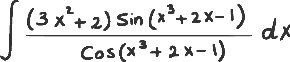
\includegraphics{imagen/formula.pdf}
\end{figure}

\noindent
es m�s natural que escribir en \LaTeX:
\vspace*{-1ex}
\begin{footnotesize}\begin{verbatim}
                    \int {\frac { \left( 3\,{x}^{2}+2 \right)
                                  \sin \left( {x}^{3}+2\,x-1 \right) }
                                { \cos \left( {x}^{3}+2\,x-1 \right) }
                         } ~ dx
\end{verbatim}\end{footnotesize}


En el campo de reconocimiento de escritura matem�tica hay un n�mero de desaf�os a sortear. A nivel de \textbf{s�mbolos}, existen muchos que son similares y no existe un alfabeto peque�o como lo tiene un lenguaje natural. A nivel de \textbf{entrada}, la segmentaci�n de s�mbolos matem�ticos es considerablemente m�s complicada. A nivel de construcci�n de \textbf{f�rmulas v�lidas}, el texto por naturaleza es unidimensional pero expresiones matem�ticas son bidimensionales, haciendo dif�cil determinar una l�nea de referencia (\textit{baseline}) apropiada. A nivel del \textbf{renderizado}, el dibujado de s�mbolos matem�ticos no es trivial. A nivel de \textbf{interacci�n}, el stylus es un dispositivo nuevo y la interacci�n hombre-computadora tiene que repensarse para que sea eficaz.


\subsubsection*{An�lisis estructural}

Como la entrada se espera que sea matem�tica, adem�s de reconocer cada caracter individualmente, tambi�n se tienen que interpretar su posici�n y rol en la expresi�n, ver figura \ref{fig:layout_trees}.
\begin{figure}[!htbp]
    \centering
%     \vspace*{-0.2cm}
    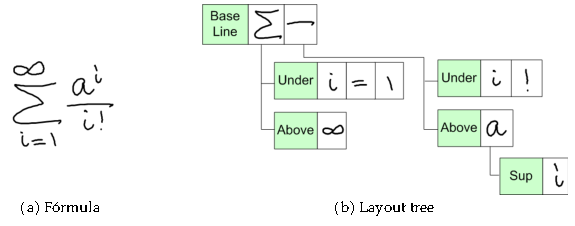
\includegraphics{imagen/layout_trees.pdf}
%     \vspace*{-0.3cm}
    \caption{Representaci�n de la f�rmula manuscrita y su correspondiente Layout.}
    \label{fig:layout_trees}
\end{figure}



\subsection{Reconocimiento de firmas}
Un campo muy interesante, donde se podr�a aplicar los m�todos mencionados en este trabajos, es el de verificaci�n de firma. Pueden verse ejemplos de firma en \ref{fig:firmas}. Se intentar� utilizar las representaciones por polinomios ortogonales descripta, para determinar si caracterizan lo suficientemente bien a las firmas como para ser usadas en este campo.
    \begin{figure}[!htbp]
    \centering
    
\includegraphics[scale=0.6]{imagen/firmas.pdf}
    \caption{Ejemplos de firmas}
    \label{fig:firmas}
    \end{figure}


\subsection{Reconocimiento de partituras musicales}
Otra aplicaci�n a considerar es el reconocimiento de notaci�n musical, como puede verse en la figura \ref{fig:partitura}. No se ha encontrado muchos sobre este tipo de reconocimiento usando el enfoque online.
    \begin{figure}[!htbp]
    \centering
    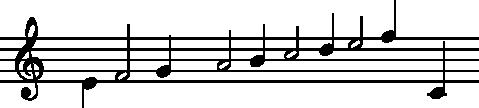
\includegraphics[scale=0.9]{imagen/Sheet_music.pdf}
    \caption{Partitura}
    \label{fig:partitura}
    \end{figure}

    \section{Resultados}

\subsection{Momentos vs Pseudo-inversa}
\subsection{Preprocesar vs No preprocesar}
\subsection{Parametrizaci�n por tiempo vs Parametrizaci�n por longitud de arco}
\subsection{Representaci�n a elegir: Legendre, Chebyshev o Legendre-Sobolev}

\subsection{Momentos como features}

\subsection{Mejor performance}
\subsection{Mejor precisi�n}

% \begin{figure}[h!]
%  \centering
%  \advance\leftskip-2.1cm
%  \advance\rightskip-2.1cm
%  \includegraphics[scale=0.42,keepaspectratio=true]{/home/spe/projects/legendre/least_square_L_without_prepocess.pdf}
% % \end{figure}
% % \begin{figure}[h!]
% %  \centering
% \hspace*{-0.4cm}
% \includegraphics[scale=0.41,keepaspectratio=true]{/home/spe/projects/legendre/least_square_L.pdf}
% \end{figure}


\bibliography{bibliografia} % indica el archivo de bibliograf�a
\bibliographystyle{pablo}   % indica el estilo de la bibliograf�a.
                            % Otros estilos (en orden de pref.): unsrt, alpha, plain, abbrv

\end{document}